\documentclass[../DoAn.tex]{subfiles}
\usepackage{graphicx}
\usepackage[utf8]{inputenc}
\usepackage{float}
\usepackage{subcaption}
\usepackage{array}
\usepackage{subfig}
\usepackage[labelfont=it]{caption}
\usepackage{fancyvrb} % Thay thế listings bằng fancyvrb
\usepackage{xcolor}

% Thiết lập đánh số hình theo chương
\numberwithin{figure}{chapter}

\captionsetup[subfigure]{
    labelfont=it,
    labelformat=simple,
    labelsep=space
}

\renewcommand{\thesubfigure}{Hình \thefigure.\arabic{subfigure}}

\begin{document}

\section{Các quy tắc chung trong ngôn ngữ lập trình Dart}
Dart hỗ trợ hai loại biên dịch đó là: Just in time (JIT) và Ahead of time (AoT). Cú pháp của nó về cơ bản là sự pha trộn của CPP, Python, Java và JavaScript.
Cú pháp là một chương trình Dart cơ bản bao gồm nhiều yếu tố khác nhau như từ khóa, mã định danh, hằng số, ký tự chuỗi, kiểu dữ liệu và ký hiệu. 

\textbf{Hàm \texttt{main} – điểm bắt đầu của chương trình:} 

Hàm \texttt{main} trong Dart có thể được định nghĩa \textbf{không có tham số} hoặc \textbf{có tham số} truyền vào. Cụ thể, nếu chương trình không cần nhận tham số từ bên ngoài, ta định nghĩa hàm \texttt{main} đơn giản như sau:

\begin{lstlisting}
void main() {
  // Code here ...
}    
\end{lstlisting}

Ngược lại, nếu muốn truyền tham số (ví dụ các đối số dòng lệnh) cho chương trình, ta có thể khai báo \texttt{main} với một danh sách tham số kiểu chuỗi:
\begin{lstlisting}
void main(List<String> args) {
  // ...
}
\end{lstlisting}

Ở ví dụ trên, \texttt{List<String> args} là tham số tùy chọn, chứa danh sách các chuỗi nhập vào chương trình (ví dụ khi chạy ứng dụng từ dòng lệnh). Kiểu trả về của \texttt{main} luôn là \texttt{void} (hàm không trả về giá trị).

Như vậy, Dart cho phép linh hoạt trong khai báo hàm \texttt{main}: có thể có hoặc không có tham số. Tuy nhiên, trong cả hai trường hợp, hàm \texttt{main} chỉ được gọi một lần khi chương trình khởi động và kết thúc khi toàn bộ chương trình kết thúc. Người lập trình cần phải đảm bảo mọi logic khởi chạy ứng dụng đều được gọi trực tiếp hoặc gián tiếp từ hàm \texttt{main} này,

\textbf{Phân biệt chữ hoa và chữ thường trong tên:} 

Dart là ngôn ngữ phân biệt chữ hoa và chữ thường (case-sensitive). 

Các định danh (tên biến, hàm, lớp,...) được viết khác nhau về chữ hoa/chữ thường sẽ được hiểu là những định danh hoàn toàn độc lập. 

Ví dụ, \texttt{MyVariable} và \texttt{myVariable} được coi là hai tên khác nhau trong Dart.

Do đó, người lập trình cần phải thống nhất trong cách đặt tên biến, tránh gây nhầm lẫn giữa các biến, hàm,... 

\textbf{Kết thúc lệnh bằng dấu chấm phẩy:} 

Tương tự nhiều ngôn ngữ C-like khác, mỗi câu lệnh trong Dart phải kết thúc bằng dấu chấm phẩy (\texttt{;}). Dấu chấm phẩy đóng vai trò phân tách các lệnh liên tiếp trong mã nguồn.  

Khi trình biên dịch Dart đọc mã, dấu \texttt{;} cho biết đây là điểm kết thúc của một lệnh. Nếu thiếu dấu chấm phẩy ở cuối một lệnh, mã nguồn sẽ không hợp lệ và gây lỗi cú pháp. 

Ví dụ, giả sử ta viết hai lệnh nối tiếp mà quên dấu \texttt{;} ở giữa:
\begin{lstlisting}
    print('Hello')
    print('World')
\end{lstlisting}

Ở tình huống này, trình biên dịch sẽ không thể hiểu được ranh giới giữa hai lệnh \texttt{print} và sẽ báo lỗi. Vì vậy cần phải sửa bằng cách thêm \texttt{;} để ngăn cách giữa các lệnh: 
\begin{lstlisting}
    print('Hello');
    print('World');
\end{lstlisting}

\textbf{Khối lệnh và cặp dấu ngoặc nhọn:} 

Một nhóm các lệnh liên tiếp được nhóm lại với nhau tạo thành một khối lệnh (block). Trong Dart cũng như trong nhiều ngôn ngữ lập trình khác, khối lệnh được bao bọc bởi cặp dấu ngoặc nhọn mở và đóng. Mục đích của khối lệnh là để gộp nhiều câu lệnh thành một đơn vị logic, chẳng hạn nội dung của một hàm, hoặc thân của một câu lệnh điều kiện \texttt{if}/\texttt{else}, hoặc thân vòng lặp \texttt{for}/\texttt{while}. 

Mỗi khi bắt đầu một khối lệnh mới, ta dùng dấu \texttt{\{} và khi kết thúc khối đó, ta dùng dấu \texttt{\}}. Các khối lệnh có thể lồng nhau: bên trong một khối lệnh có thể chứa thêm các khối lệnh con (ví dụ: bên trong hàm \texttt{main} có khối lệnh của một vòng lặp, trong vòng lặp lại có khối lệnh của một cấu trúc điều kiện, v.v.). 

Việc thụt lề (indentation) thường được sử dụng khi viết mã để cho thấy trực quan các khối lệnh nằm trong nhau, giúp người đọc dễ theo dõi cấu trúc chương trình.

\begin{lstlisting}
if (a > 1) {
    // Nested code blocks are allowed
    if (...) {
        // Block 1
    } else {
        // Block 2
    }
} else {
    // Alternative block
}
\end{lstlisting}

Trong thực tế, nếu khối lệnh chỉ có duy nhất một lệnh bên trong, Dart cho phép người lập trình bỏ cặp ngoặc nhọn và viết trực tiếp lệnh đó sau cấu trúc điều khiển.
\begin{lstlisting}
    if (x > 0) print('x is positive');
\end{lstlisting}

Dart khuyến khích để mã nguồn rõ ràng và tránh các lỗi logic do nhầm lẫn phạm vi của khối lệnh.

\textbf{Chú thích trong mã nguồn:} 

\textbf{Chú thích} là phần nội dung trong mã nguồn mà trình biên dịch sẽ \textbf{bỏ qua không thực thi}, thường được dùng để giải thích code hoặc tạm thời vô hiệu hóa một đoạn mã. Dart hỗ trợ cả chú thích một dòng và chú thích nhiều dòng, tương tự như ngôn ngữ C/C++. 

\begin{itemize}
\item \textbf{Chú thích trên một dòng:} 
    
Bắt đầu bằng ký tự //. Tất cả nội dung sau // trên cùng một dòng sẽ được coi là chú thích và bị bỏ qua khi chạy chương trình. 

\textit{Ví dụ:}
\begin{lstlisting}
// This line is ignored (a comment)
print('Hello');  // Prints 'Hello'
\end{lstlisting}
Ở ví dụ trên, dòng đầu tiên hoàn toàn là chú thích, còn ở dòng thứ hai, phần từ // trở đi ("// Prints 'Hello'") cũng là chú thích (giải thích cho lệnh \texttt{print})

 \item \textbf{Chú thích trên nhiều dòng: } 
 
 Bắt đầu bằng /* và kết thúc bằng */. Mọi nội dung nằm giữa cặp /* và */ sẽ được coi là chú thích. Kiểu chú thích này cho phép ghi chú trải trên nhiều dòng. 
 
\textit{Ví dụ:}
\begin{lstlisting}
/* 
Calculate the area of a circle.
Radius r = 5.
*/
double area = 3.14 * 5 * 5;
\end{lstlisting}

Tất cả những dòng văn bản giữa /* và */ ở trên đều là chú thích và sẽ bị bỏ qua khi chương trình chạy. 
Ngoài ra, Dart cho phép lồng các chú thích nhiều dòng bên trong nhau.

\end{itemize}

Ngoài hai loại chú thích trên, Dart còn hỗ trợ \textbf{chú thích tài liệu} (documentation comments). Đây là các chú thích đặc biệt dùng để tự động sinh tài liệu API cho code, bắt đầu bằng /// (ba dấu gạch chéo) cho mỗi dòng chú thích đơn, hoặc cặp /** ... */ cho chú thích nhiều dòng dạng tài liệu. 

\textit{Ví dụ:} 
\begin{lstlisting}
/// Calculate factorial of positive integer n.
/// return n! (1 * 2 * ... * n).
int factorial(int n) { ... }    
\end{lstlisting}

Các chú thích bắt đầu bằng /// như trên sẽ được các công cụ tạo tài liệu (vd. dartdoc) hiểu và trích xuất thành phần mô tả cho hàm \texttt{factorial}. Mặc dù chú thích tài liệu được đặt trong mã nguồn, chúng không ảnh hưởng đến việc biên dịch chương trình, tương tự như các chú thích thông thường.

\textbf{Quy tắc định danh:}

Mọi định danh (tên biến, tên hàm, tên lớp, v.v.) trong Dart phải tuân thủ quy tắc đặt tên giống như nhiều ngôn ngữ lập trình khác. Cụ thể, định danh phải bắt đầu bằng một ký tự chữ cái (a–z hoặc A–Z) hoặc dấu gạch dưới {\_}, và các ký tự tiếp theo có thể là chữ cái hoặc chữ số. Định danh không được phép bắt đầu bằng chữ số, không được chứa khoảng trắng hay các ký tự đặc biệt (ngoại trừ ký tự gạch dưới, và cả ký hiệu {\$} cũng được cho phép sử dụng trong định danh). Ngoài ra, không được dùng các từ khóa dành riêng của Dart làm tên định danh. 

\textit{Ví dụ:} 
\begin{itemize}
    \item \texttt{MyClass}, \texttt{{\_}result123} là các \textbf{định danh hợp lệ.} 
    \item \texttt{123number} (bắt đầu bằng chữ số) và \texttt{username} (chứa ký tự không hợp lệ là dấu (-) là những \textbf{định danh không hợp lệ}.
\end{itemize}

Về quy ước đặt tên nhằm viết mã nhất quán và dễ đọc, Dart tuân thủ phong cách \textit{camelCase}/\textit{PascalCase}: Tên biến, hàm, và thuộc tính thường được viết dưới dạng \textit{camelCase} (chữ cái đầu tiên viết thường, các chữ cái đầu của những từ tiếp theo viết hoa), còn tên lớp, tên enum thì viết dưới dạng \textit{PascalCase} (viết hoa chữ cái đầu của mỗi từ) theo khuyến nghị của hướng dẫn Effective Dart. 

\textit{Ví dụ:} 
\begin{itemize}
    \item \textbf{\texttt{DataRepository}} phù hợp khi đặt tên lớp vì nó tuân theo PascalCase. 
    \item \textbf{\texttt{isValid}, \texttt{calculateSum}} phù hợp khi đặt tên biến vì tuân theo camelCase.
\end{itemize}

Việc tuân theo các quy tắc và quy ước định danh này giúp mã Dart rõ ràng, dễ hiểu và tránh được lỗi khi biên dịch. 

\textbf{Mọi thứ trong Dart là đối tượng:} 

Dart là ngôn ngữ hướng đối tượng thuần túy, nghĩa là \textbf{mọi thứ} có thể gán cho biến đều là đối tượng. Số nguyên, số thực, chuỗi, giá trị boolean, thậm chí cả hàm cũng đều được coi là đối tượng (thể hiện bởi các lớp như int, double, String, bool, Function, ...). Đặc biệt, ngay cả giá trị \textbf{null} cũng được biểu diễn như một đối tượng thuộc kiểu Null trong Dart (trước khi có null-safety, null là một đối tượng hợp lệ). 

Mỗi đối tượng trong Dart là một thể hiện của một lớp nào đó, và tất cả các lớp (kể cả các lớp do người dùng định nghĩa) đều ngầm định kế thừa từ một lớp cơ sở chung có tên là Object. Object là gốc của mọi lớp trong hệ thống loại của Dart. Mọi đối tượng Dart đều chia sẻ một số phương thức cơ bản từ Object:
\begin{itemize} 
\item \textbf{\texttt{hashCode}} – Thuộc tính trả về mã băm (hash code) của đối tượng 

Thuộc tính \texttt{hashCode} trả về một số nguyên đại diện cho trạng thái của đối tượng, được sử dụng trong các cấu trúc dữ liệu dựa trên băm như Set và Map. Mã băm mặc định được triển khai trong lớp Object chỉ phản ánh danh tính (identity) của đối tượng. 

Khi ghi đè toán tử \texttt{==} để so sánh các đối tượng dựa trên trạng thái (tức là các thuộc tính), cần ghi đè thuộc tính \texttt{hashCode} để đảm bảo rằng hai đối tượng được coi là bằng nhau sẽ có cùng mã băm. 

\item \textbf{\texttt{toString()}} – Phương thức toString() 

Phương thức \texttt{toString()} trả về một chuỗi mô tả đối tượng, thường được sử dụng để hiển thị thông tin trong quá trình gỡ lỗi hoặc ghi log. Mặc định, \texttt{toString()} trả về chuỗi dạng Instance of 'ClassName', điều này không cung cấp nhiều thông tin hữu ích. Do đó, người ta thường ghi đè phương thức này để trả về chuỗi mô tả chi tiết hơn về đối tượng. 

\textit{Ví dụ:}
\begin{lstlisting}
class Person { 
    final String name; 
    final int age;
    
    Person(this.name, this.age);
    
    @override String toString() 
    => 'Person(name: $name, age: $age)'; 
} 
\end{lstlisting}
Với cách ghi đè này, khi in một đối tượng Person ta sẽ nhận được kết quả rõ ràng, tường minh: 
    \texttt{Person(name: Alice, age: 30)}
\item \textbf{Toán tử \texttt{==}} – So sánh đối tượng 

Toán tử \texttt{==} được sử dụng để so sánh hai đối tượng. Mặc định, Dart so sánh hai đối tượng dựa trên danh tính, tức là chúng phải là cùng một đối tượng trong bộ nhớ để được coi là bằng nhau. Hai đối tượng nếu có giá trị giống nhau nhưng không cùng danh tính thì khi sử dụng toán tử \texttt{==} trả về kết quả \textbf{False}. 

Để so sánh các đối tượng dựa trên giá trị, cần ghi đè toán tử \texttt{==} và thuộc tính \texttt{hashCode}
\end{itemize}

\textbf{Từ khóa public/private/protected}: 

Dart không sử dụng các từ khóa như \texttt{public}, \texttt{private} hay \texttt{protected} để quy định phạm vi truy cập như trong một số ngôn ngữ hướng đối tượng khác (ví dụ Java, C++). Mặc định, mọi lớp, thuộc tính và phương thức được khai báo trong Dart đều có phạm vi truy cập “công khai” đối với các đoạn mã khác, trừ khi được định nghĩa đặc biệt để giới hạn phạm vi. Nếu không làm gì thêm, các thành phần định nghĩa có thể được truy cập từ bất kỳ đâu. 

Thiết kế của Dart đơn giản hóa việc đóng gói khi cho rằng thành phần nào không được đánh dấu riêng tư thì sẽ được hiểu là công khai. Điều này giúp loại bỏ sự rườm rà khi phải chỉ định \texttt{public} cho từng thành phần, đồng thời khuyến khích lập trình viên suy nghĩ về việc tổ chức mã theo thư viện (library) để kiểm soát truy cập thay vì dựa vào từ khóa.

\textbf{Cách khai báo private bằng dấu {\textbf{\_}}}: 

Thay vì dùng từ khóa, Dart quy định phạm vi riêng tư (private) ở cấp thư viện thông qua quy ước đặt tên: Nếu tên định danh bắt đầu bằng dấu gạch dưới \_ thì định danh đó được xem là private trong library. Các thành viên (thuộc tính, phương thức) hoặc các khai báo (biến, hàm, lớp) có tên bắt đầu bằng \_ chỉ có thể được truy cập ở trong cùng một thư viện (thông thường là cùng một file .dart). Ngược lại, nếu tên không bắt đầu bằng \_ thì thành phần đó là công khai và có thể được truy cập từ bất cứ đâu sau khi import. 

\textbf{Ví dụ:} Giả sử có lớp Person được định nghĩa như sau: 
\begin{lstlisting}
class Person {
  String _name; // private property
  int age;      // public property

  Person(this._name, this.age);
}
\end{lstlisting}

Trong ví dụ trên: 
\begin{itemize}
    \item Thuộc tính {\texttt{\_name}} là một thuộc tính private của lớp Person. Điều này đồng nghĩa {\texttt{\_name}} chỉ có thể được truy cập hoặc sửa đổi bởi mã nằm trong cùng library định nghĩa lớp Person (ví dụ bên trong chính file khai báo Person hoặc các file khác dùng part of chung thư viện), và không thể truy cập trực tiếp từ một library khác. 
    \item Ngược lại, thuộc tính \texttt{age} không có dấu gạch dưới đầu tên nên được coi là công khai – code từ module khác (sau khi import thư viện chứa Person) có thể đọc/ghi \texttt{age} tùy ý.
\end{itemize}

Quy tắc dùng dấu gạch dưới để đánh dấu private giúp mã Dart ngắn gọn hơn (vì không cần từ khóa) nhưng vẫn đảm bảo đóng gói thông tin: mọi chi tiết triển khai nội bộ mà lập trình viên muốn giấu đều chỉ cần đặt tên bắt đầu bằng \_ là đủ.

\section{Biến, hằng, kiểu dữ liệu}
Trong ngôn ngữ lập trình Dart, mỗi giá trị đều có một \textbf{kiểu dữ liệu} xác định, và tất cả những giá trị có thể gán vào biến đều là \textbf{đối tượng}
(kể cả các giá trị cơ bản như số, chuỗi, hay \texttt{null}). Các kiểu dữ liệu cơ bản có sẵn trong Dart bao gồm: \textbf{\texttt{int}} (số nguyên, 64-bit), \textbf{\texttt{double}} (số thực dấu phẩy động kép, 64-bit), \textbf{\texttt{String}} (chuỗi ký tự Unicode), \textbf{\texttt{bool}} (kiểu luận lý, với hai giá trị \texttt{true}/\texttt{false}), v.v. Ngoài ra còn có các kiểu tổng quát như \texttt{Object} (kiểu gốc của mọi đối tượng) và \texttt{dynamic} (kiểu động). 

\subsection{Khai báo biến} 
Dart là ngôn ngữ kiểm tra kiểu tĩnh (\textit{statically-typed}), tức là mỗi biến trong chương trình đều mang một kiểu dữ liệu cố định ngay từ khi khai báo. Tuy nhiên, Dart hỗ trợ \textit{suy luận kiểu} nên ta không nhất thiết phải chỉ rõ kiểu dữ liệu khi khai báo biến. Cụ thể, để khai báo một biến, ta có thể dùng từ khóa \textbf{\texttt{var}} theo cú pháp: 
\begin{lstlisting}
    var <variable_name> = <value_expression>;
\end{lstlisting}

Khi sử dụng \texttt{var}, trình biên dịch Dart sẽ tự động suy ra kiểu dữ liệu của biến dựa trên giá trị được gán ban đầu. Ví dụ: 
\begin{lstlisting}
    var name = 'Alice'; // Dart infers this as String
    var age = 25;  // Dart infers this as int
\end{lstlisting}

Trong ví dụ trên, biến \texttt{a} được gán một chuỗi ký tự, nên Dart hiểu \texttt{a} thuộc kiểu \texttt{String}. Sau khi khai báo, \texttt{a} chỉ có thể nhận các giá trị kiểu \texttt{String}; nếu cố gán một kiểu khác (ví dụ số nguyên) cho \texttt{a} thì chương trình sẽ báo lỗi kiểu (\textit{type error}) khi biên dịch.  

Dart cũng cho phép khai báo biến với kiểu dữ liệu tường minh thay vì sử dụng \texttt{var}. Người lập trình có thể chỉ định trực tiếp kiểu dữ liệu trước tên biến. Ví dụ:

\begin{lstlisting}
String s = "String";  // Variable s of type String
int i = 5; // Variable i of type integer
double d = 1.1234;  // Variable d of type double
bool b = true; // Variable b of type boolean
\end{lstlisting}

Việc khai báo rõ kiểu dữ liệu như trên giúp mã nguồn rõ ràng về mục đích sử dụng biến, và trình biên dịch sẽ kiểm tra để đảm bảo biến chỉ được gán các giá trị thuộc đúng kiểu đó. Ngược lại, sử dụng \texttt{var} đem lại sự tiện lợi và ngắn gọn, đặc biệt khi kiểu dữ liệu có thể dễ dàng suy ra từ biểu thức gán. Trong thực tế, ta có thể chọn cách khai báo tùy tình huống, nhưng cần nhất quán và dễ đọc. 

Trong trường hợp cần một biến có thể chấp nhận nhiều loại giá trị khác nhau, Dart cung cấp kiểu đặc biệt \textbf{\texttt{dynamic}}. Khi một biến được khai báo là \texttt{dynamic}, nghĩa là quá trình kiểm tra kiểu tại biên dịch sẽ được nới lỏng: biến đó có thể nhận bất kỳ kiểu dữ liệu nào trong lúc chạy, và mọi kiểm tra về tính hợp lệ kiểu sẽ dời đến thời gian chạy (\textit{runtime}). 

\textit{Ví dụ:} 
\begin{lstlisting}
dynamic dyn = 123; // Initialize dyn as an integer
dyn = "Dynamic"; // dyn is reassigned to a string
dyn = 1.12345; // dyn is reassigned to a double
\end{lstlisting}

Ở ví dụ trên, cùng một biến \texttt{dyn} lần lượt được gán số nguyên, chuỗi và số thực mà không gây lỗi biên dịch. Tuy nhiên, việc sử dụng \texttt{dynamic} cũng tiềm ẩn rủi ro: vì trình biên dịch không kiểm tra chặt chẽ kiểu, nên các lỗi do gán sai kiểu chỉ được phát hiện khi chạy chương trình, có thể dẫn đến ngoại lệ nếu ta gọi một phương thức không phù hợp với kiểu thực sự của giá trị. Do đó, \textbf{chỉ nên dùng \texttt{dynamic} khi thật sự cần thiết}, trong các tình huống linh hoạt đặc biệt; còn nhìn chung, với các biến có kiểu xác định, nên dùng \texttt{var} (kết hợp suy luận kiểu) hoặc khai báo kiểu tường minh để tận dụng kiểm tra lỗi ngay từ lúc biên dịch. 

\subsection{Khai báo hằng} 
Bên cạnh biến thay đổi được, Dart cho phép khai báo \textit{hằng} – tức biến chỉ đọc, không thể thay đổi giá trị sau khi đã được khởi tạo. Để khai báo hằng, ta sử dụng từ khóa \textbf{\texttt{final}} hoặc \textbf{\texttt{const}} (có thể dùng thay cho \texttt{var}, và cũng có thể kèm kiểu dữ liệu hoặc không). 

\textit{Ví dụ:} 
\begin{lstlisting}
const constantName = value_expression;
final name1 = value_expression;
// You can also specify the type explicitly
final String name2 = value_expression;
\end{lstlisting}

Cả \texttt{final} và \texttt{const} đều tạo ra một biến chỉ được gán một lần duy nhất. Sự khác biệt chính giữa chúng là thời điểm và cách thức giá trị của biến được xác định: 
\begin{itemize}
  \item \textbf{\texttt{final}} – Biến được khai báo với \texttt{final} là một hằng chỉ đọc tại \textit{thời gian chạy}. Điều này có nghĩa là ta có thể gán giá trị cho nó một lần duy nhất, nhưng giá trị đó có thể được tính toán hoặc lấy từ một biểu thức khi chương trình chạy. Khi đã gán rồi, biến \texttt{final} không thể thay đổi (mọi cố gắng gán lần thứ hai sẽ gây lỗi). Ví dụ, ta có thể viết \texttt{final x = DateTime.now();} để lấy thời điểm hiện tại làm giá trị, và \texttt{x} sẽ giữ nguyên giá trị đó suốt thời gian chạy chương trình.
  \item \textbf{\texttt{const}} – Biến khai báo với \texttt{const} là một \textit{hằng số tại thời điểm biên dịch} (compile-time constant). Điều này đòi hỏi giá trị gán cho \texttt{const} phải được biết chắc chắn và cố định ngay trong mã nguồn (ví dụ: các literal hoặc biểu thức hằng). Nói cách khác, \textbf{một biến \texttt{const} bắt buộc phải nhận một biểu thức có thể đánh giá tại thời điểm biên dịch}. Các biến \texttt{const} cũng mang tính chất \textit{bất biến} giống final (không thể thay đổi sau khi gán), và trên thực tế biến \texttt{const} cũng được xem là \texttt{final} ngầm định. Tuy nhiên, vì yêu cầu giá trị cố định sẵn, \texttt{const} thường được dùng cho các hằng số đơn giản hoặc để tạo ra các đối tượng bất biến tại compile-time.
\end{itemize}

Dưới đây là ví dụ minh họa cách sử dụng \texttt{const} và \texttt{final}: 

\begin{lstlisting}
// Constant, value = 120 (determined at compile time)
const int minutes = 2 * 60;   

// Get a random number (0..499)
var randomNumber = Random().nextInt(500);    

// Final constant, value determined at runtime
final result = randomNumber * 2;        

// Cannot use const because the expression is not a compile-time constant
const wrongResult = randomNumber * 2;  
\end{lstlisting}

Giải thích: 
Trong đoạn mã trên \texttt{minutes} là hằng số tính sẵn (2 * 60 được tính toán ngay khi biên dịch, cho ra 120); ngược lại, \texttt{result} được khai báo \texttt{final} và nhận giá trị là kết quả phép tính với một số ngẫu nhiên sinh ra lúc chạy chương trình. Ta \textbf{không thể} dùng \texttt{const} trong trường hợp giá trị gán không phải hằng số xác định sẵn(dòng lệnh cuối).

\subsection{Các kiểu dữ liệu} 
Dart hỗ trợ các kiểu dữ liệu cơ bản như \textbf{bool, int, double, String, List, Set và Map}. Mỗi kiểu dữ liệu biểu diễn một loại thông tin khác nhau, có miền giá trị và đặc điểm riêng.

\begin{table}[h]
\centering
\begin{tabular}{|p{0.2\textwidth}|p{0.75\textwidth}|}
\hline
\textbf{Kiểu dữ liệu} & \textbf{Mô tả} \\ \hline
\textbf{bool} & Kiểu logic (Boolean), chỉ có hai giá trị: \texttt{true} (đúng) hoặc \texttt{false} (sai). \\ \hline
\textbf{int} & Kiểu số nguyên (integer), biểu diễn các số nguyên (có dấu) trong khoảng 64-bit. \\ \hline
\textbf{double} & Kiểu số thực dấu phẩy động (double precision), độ chính xác kép 64-bit, biểu diễn số thực (số có phần thập phân). \\ \hline
\textbf{String} & Kiểu chuỗi ký tự (string), biểu diễn một dãy các ký tự Unicode (UTF-16). Khai báo bằng cặp dấu nháy đơn hoặc nháy kép. \\ \hline
\textbf{List (Danh sách)} & Cấu trúc danh sách (list) các phần tử, tương tự mảng một chiều. Các phần tử có thứ tự tuyến tính và được truy cập bằng chỉ số (index). \\ \hline
\textbf{Set (Tập hợp)} & Cấu trúc tập hợp (set) các phần tử không trùng lặp. Không duy trì thứ tự cố định của phần tử, dùng để lưu các giá trị duy nhất. \\ \hline
\textbf{Map (Ánh xạ)} & Cấu trúc ánh xạ (map) gồm các cặp khóa - giá trị (key - value). Mỗi khóa ánh xạ tới một giá trị, cho phép tra cứu giá trị thông qua khóa. \\ \hline
\end{tabular}
\caption{Mô tả các kiểu dữ liệu cơ bản trong Dart}
\end{table}

\subsubsection{Bool} 
Dart cung cấp hỗ trợ sẵn có cho kiểu dữ liệu Boolean. Kiểu dữ liệu Boolean trong DART chỉ hỗ trợ hai giá trị true và false. Từ khóa bool được sử dụng để biểu diễn một ký tự Boolean trong DART. 

\textit{Ví dụ:} 
\begin{lstlisting}
void main() { 
   bool test; 
   test = 12 > 5; 
   print(test); 
}
\end{lstlisting}

Trong ví dụ trên, \texttt{test} là các biến \texttt{bool}. Biểu thức so sánh 12 > 5 sẽ quyết định giá trị của biến \texttt{test}. Câu lệnh \texttt{print(test)} sẽ trả ra kết quả true.

\subsubsection{Int}
\textbf{int} (viết tắt của integer) là kiểu dữ liệu số nguyên trong Dart, dùng để biểu diễn các số nguyên (không có phần thập phân). Miền giá trị của \texttt{int} trong Dart rất lớn: trên các nền tảng thông thường, \texttt{int} là số nguyên 64-bit có dấu, giá trị nhỏ nhất khoảng $-2^{63}$ và lớn nhất khoảng $2^{63}-1$ (tức khoảng từ $-9.22\times10^{18}$ đến $9.22\times10^{18}$).

Cú pháp khai báo một số nguyên kiểu \texttt{int}: 

\begin{lstlisting}
int var_name // Declare an integer
\end{lstlisting}

\textit{Ví dụ:} 
\begin{lstlisting}
void main() {
   // declare an integer
   int num1 = 10;             
   // print value
   print(num1);
}
\end{lstlisting}
Khi chạy chương trình, kết quả in ra là \textbf{10}

\subsubsection{Double}  
\textbf{double} là kiểu dữ liệu số thực dấu phẩy động trong Dart, dùng để biểu diễn các số có phần thập phân (số thực). Kiểu \texttt{double} chiếm 64-bit và tuân theo tiêu chuẩn IEEE 754 (độ chính xác kép).
Cú pháp khai báo một số thực kiểu \texttt{double}: 
\begin{lstlisting}
    double var_name // Declare a double value
\end{lstlisting}

\textit{Ví dụ:}
\begin{lstlisting}
void main() {
   // Declare a double value
   double num1 = 12.34;             
   // print value:
   print(num1);
}
\end{lstlisting}

Khi chạy chương trình, kết quả in ra là \textbf{12.34}.
\subsubsection{String} 

\textbf{String} là kiểu dữ liệu chuỗi ký tự trong Dart, dùng để biểu diễn văn bản (text). Mỗi chuỗi là một dãy các ký tự thuộc bảng mã Unicode (mỗi ký tự được mã hóa dưới dạng một hoặc hai byte UTF-16). Kiểu \texttt{String} trong Dart là một lớp đối tượng (thuộc \texttt{dart:core}), và giống như nhiều ngôn ngữ khác, chuỗi trong Dart là \textbf{bất biến} (immutable), tức là giá trị chuỗi không thể thay đổi sau khi được tạo ra. Mọi thao tác "thay đổi" trên chuỗi thực chất sẽ tạo ra một chuỗi mới. 

Để tạo một chuỗi ký tự, ta đặt nội dung chuỗi trong cặp dấu nháy đơn (\texttt{'...'}) hoặc nháy kép (\texttt{"..."}). Dart cho phép sử dụng linh hoạt cả hai loại dấu nháy để thuận tiện khi chuỗi bản thân có chứa dấu nháy. 

Một số thuộc tính và phương thức thông dụng của \texttt{String} bao gồm:
\begin{itemize}
\item \texttt{.length}: Trả về độ dài chuỗi
\item \texttt{.toUpperCase()} / \texttt{toLowerCase()}: Dùng để chuyển chuỗi thành chữ hoa / chữ thường
\item \texttt{.contains()} : Dùng để kiểm tra chuỗi có chứa một chuỗi con
\item \texttt{.substring(start, [end])}: Dùng để trích xuất chuỗi con từ chuỗi cho trước, bắt đầu từ vị trí \texttt{start} đến hết vị trí.  \texttt{end - 1}. Nếu không có \texttt{[end]} thì mặc định cắt đến hết xâu.
\item \texttt{.compareTo(str)}: So sánh chuỗi theo thứ tự từ điển, trả về -1/0/1 tương ứng với nhỏ hơn, bằng, lớn hơn.
\end{itemize}

\textit{Ví dụ:} 
\begin{lstlisting}
var s1 = "abcdef"; 
print (s1.length);
// Output: 6

var s2 = "phuc";
print(s2.toUpperCase()); 
// Output: PHUC

var s3 = "abcdefghi";
print(s3.substring(1, 4));
// Output: abc

var s4 = "helloiamkhanh";
print(s4.contains("khanh");
// Output: true

var s5 = "abcde";
print(s5.compareTo("bcdef"));
// Output: -1
\end{lstlisting}

\subsubsection{List} 
\textbf{List} là cấu trúc dữ liệu dạng danh sách tuyến tính các phần tử trong Dart, tương tự như mảng (array) một chiều trong các ngôn ngữ khác. Mỗi phần tử trong \texttt{List} đều có một vị trí chỉ số (index) xác định, bắt đầu từ 0. Phần tử đầu tiên của list có chỉ số 0, phần tử thứ hai chỉ số 1, v.v., và phần tử cuối cùng có chỉ số \texttt{length - 1} (trong đó \texttt{length} là độ dài danh sách). List duy trì thứ tự sắp xếp phần tử theo trình tự thêm vào.
\begin{itemize}
\item Nếu khai báo \textbf{List} với kiểu dữ liệu cụ thể, thì tất cả các phần tử trong List phải có kiểu dữ liệu đó. 

\textit{Ví dụ:} 
\begin{lstlisting}
// Valid
List<int> numbers = [1, 2, 3];

// Error: 'a' is not of type int
List<int> invalidNumbers = [1, 'a', 3];  
\end{lstlisting}

\item Nếu khai báo \textbf{List<dynamic>} hoặc \textbf{không chỉ định kiểu}, Dart cho phép các phần tử có kiểu khác nhau.

\textit{Ví dụ:}
\begin{lstlisting}
// Allowed because the list is declared as dynamic
List<dynamic> mixedList = [1, 'hello', true, 3.14];
var anotherList = [1, 'abc', 2.5];
\end{lstlisting}

\end{itemize}

Có hai loại list: \textbf{List cố định độ dài} và \textbf{List có thể thay đổi độ dài (growable)}. 

Danh sách có chiều dài cố định \textbf{không thể} thay đổi số lượng phần tử sau khi được khởi tạo. 

Ví dụ List có độ dài cố định:
\begin{lstlisting}
List<String> myList = List<String>(3);
myList[0] = 'one';
myList[1] = 'two';
myList[2] = 'three';
// myList.add('four'); -> Error
\end{lstlisting}

Danh sách có thể mở rộng \textbf{cho phép} {thay đổi số lượng} phần tử. 

Ví dụ List có thể mở rộng:
\begin{lstlisting}
List<int> myList = List<int>();
myList.add(42);
myList.add(2023);
print(myList); // [42, 2023]
print(myList.length); // 2

myList.add(2024);
print(myList); // [42, 2023, 2024]
print(myList.length); // 3
\end{lstlisting}

Một số thuộc tính và phương thức phổ biến của List: 
\begin{itemize}
\item \texttt{.length}: Trả về số phần tử có trong danh sách
\item \texttt{.index}: Dùng để truy cập vào phần tử có vị trí \texttt{index} trong list
\item \texttt{.add(value)}: Dùng để thêm giá trị \texttt{value} vào cuối danh sách.
\item \texttt{.removeAt(int index)}: Dùng để xóa phần tử ở vị trí index trong danh sách.
\item \texttt{.removeLast()}: Xóa phần tử ở vị trí cuối cùng trong danh sách.
\item \texttt{.clear()}: Xóa tất cả các phần tử trong danh sách.
\end{itemize}

\textit{Ví dụ:} 
\begin{lstlisting}
var arr = [1, 12, 4, 26, 9, 2, 'u', 'i', 'a'];
print(arr.length); // Output: 9
print(arr[0]); // Output: 1

// Add an element to the List
arr.add(10);
print(arr);
// Output: [1, 12, 4, 26, 9, 2, 'u', 'i', 'a', 10]

// Remove an element by value
arr.remove('a');
print(arr);
// Output: [1, 12, 4, 26, 9, 2, 'u', 'i', 10]

// Remove an element by index
arr.removeAt(0);
print(arr);
// Output: [12, 4, 26, 9, 2, 'u', 'i', 10]

// Remove the last element in the List
arr.removeLast();
print(arr);
// Output: [12, 4, 26, 9, 2, 'u', 'i']

// Remove all elements from the List
arr.clear();
print(arr);
// Output: []
\end{lstlisting}
\subsubsection{Set}
\textbf{Set} (Tập hợp) là một cấu trúc dữ liệu lưu trữ các phần tử không trùng lặp. Khác với \texttt{List}, \texttt{Set} không duy trì thứ tự các phần tử dựa trên vị trí chỉ số; thay vào đó, \texttt{Set} được tổ chức như một tập hợp toán học, mỗi giá trị xuất hiện tối đa một lần và thứ tự duyệt có thể khác với thứ tự thêm. 

Trong \texttt{Set}, vì không có chỉ số, ta không truy cập phần tử theo vị trí như list. Thay vào đó, có thể dùng vòng lặp hoặc các phương thức như \texttt{contains(element)} để kiểm tra sự có mặt của phần tử. 

\textbf{Set} được khai báo bằng cách sử dụng từ khóa \texttt{set}. Có 2 cách để khai báo:
\begin{lstlisting}
// Method 1: Using var keyword
var variable_name = <variable_type>{};

// Method 2: Using explicit Set declaration
Set<variable_type> variable_name = {};
\end{lstlisting}

Một số phương thức phổ biến của Set: 
\begin{itemize}
\item \texttt{.length}: Trả về số lượng phần tử trong set.
\item \texttt{.contains(element\_name)}: Kiểm tra sự tồn tại của \texttt{element\_name} trong tập hợp, trả về \texttt{true} nếu tồn tại, trả về \texttt{false} nếu không tồn tại.
\item \texttt{.remove(element\_name)}: Xóa phần tử có giá trị bằng với \texttt{element\_name} ra khỏi tập hợp.
\item \texttt{.forEach(...)}: Duyệt qua tất cả các phần tử có trong \texttt{set}.
\item \texttt{.add(value)}: Thêm phần tử có giá trị bằng với value vào \texttt{set}, nếu nó chưa tồn tại trong đó.
\item \texttt{.clear()}: Xóa hết tất cả các phần tử trong tập hợp.
\end{itemize}

\textit{Ví dụ:}
\begin{lstlisting}
var se = {5, 10, 15, 20, 25};

// Count the number of elements in the set:
print(se.length); // Result: 5

// Check if an element exists in the set:
print(se.contains(15)); // Result: true

// Remove an element with a specific value from the set:
se.remove(15);
print(se); // Result: {5, 10, 20, 25}

// Iterate through all elements in the set:
se.forEach((element) {
    print(element);
});
// Result:
// 5
// 10
// 20
// 25

// Add an element to the set if it doesn't already exist
se.add(30);
print(se); // Result: {5, 10, 20, 25, 30}

// Remove all elements from the set:
se.clear();
print(se); // Result: {}
\end{lstlisting}

\subsubsection{Map} 
\textbf{Map} (Ánh xạ khóa - giá trị) là cấu trúc dữ liệu dạng bẳng băm (hash table) trong Dart, cho phép lưu trữ các cặp \textit{key-value} (khóa và giá trị tương ứng). \texttt{Map} tương tự như \textit{dictionary} trong Python: mỗi khóa (key) duy  duy nhất ánh xạ tới một giá trị (value).
Dart cung cấp \texttt{Map<K, V>} trong đó \texttt{K} là kiểu khóa, \texttt{V} là kiểu giá trị.  Cú pháp để khai báo một \texttt{Map} sử dụng cặp dấu ngoặc nhọn \texttt{\{\}}, nhưng khác với \texttt{Set} ở chỗ mỗi phần tử là một cặp \texttt{K: V}. 

Ví dụ về khai báo một \textbf{Map} trong Dart:
\begin{lstlisting}
var gifts = {
    // Key:    Value
    'first': 'partridge',
    'second': 'turtledoves',
    'fifth': 'golden rings',
};
\end{lstlisting}
Một số phương thức phổ biến của \texttt{Map}: 
\begin{itemize}
\item \texttt{.length}: Trả về số lượng phần tử trong Map.
\item \texttt{.containsKey(key)} / \texttt{containsValue(value)}: Kiểm tra sự tồn tại của \texttt{key/ value} trong Map, trả về \texttt{true} nếu tồn tại, trả về \texttt{false} nếu không tồn tại.
\item \texttt{.remove(key)}: Xóa cặp \texttt{key, value} theo \texttt{key}.
\item \texttt{.forEach(fn)}:có thể duyệt qua \texttt{Map} bằng \texttt{forEach((k,v) \{\})}, hoặc duyệt qua \texttt{map.keys} (tập hợp các khóa) hay \texttt{map.values} (tập hợp các giá trị).
\item \texttt{[]=}: Thêm một cặp \texttt{key-value} vào Map
\item \texttt{.clear()}: Xóa hết tất cả các phần tử trong Map.
\end{itemize}

\textit{Ví dụ:} 
\begin{lstlisting}
var mp = {'a': 1, 'b': 2, 'c': 3};

// Return the number of elements in the Map:
print(mp.length); // Output: 3

// Check if a key exists in the Map:
print(mp.containsKey('b')); // Output: true

// Check if a value exists in the Map:
print(mp.containsValue(2)); // Output: true

// Remove a key-value pair by key:
mp.remove('b');
print(mp); // Output: {'a': 1, 'c': 3}

// Iterate over all key-value pairs in the Map:
mp.forEach((k, v) {
    print('Key: $k, Value: $v');
});
// Output:
// Key: a, Value: 1
// Key: c, Value: 3

// Add a new key-value pair to the Map:
mp['d'] = 4;
print(mp); // Output: {'a': 1, 'c': 3, 'd': 4}

// Remove all elements from the Map:
mp.clear();
print(mp); // Output: {}
\end{lstlisting}

\section{Các toán tử trong Dart}
Dart cung cấp một hệ thống toán tử phong phú để hỗ trợ các phép toán cơ bản và xử lý logic. Các toán tử trong Dart có thể được chia thành nhiều nhóm, bao gồm: toán tử số học, toán tử tăng giảm đơn vị, toán tử logic, toán tử so sánh và toán tử gán. 

\subsection{Toán tử số học}
Các toán tử số học trong Dart được sử dụng để thực hiện các phép tính toán trên các số nguyên (\texttt{int}) hoặc số thực (\texttt{double}). 
\begin{itemize}
\item \texttt{+}: Phép cộng.
\item \texttt{-}: Phép trừ.
\item \texttt{*}: Phép nhân.
\item \texttt{/}: Phép chia (trả về \texttt{double} ngay cả khi hai toán hạng là \texttt{int}).
\item \texttt{\%}: Phép chia lấy phần dư (modulo).
\item \texttt{\textasciitilde/}: Phép chia lấy phần nguyên (integer division).
\end{itemize}

\textit{Ví dụ:} 
\begin{lstlisting}
    int a = 7;
    int b = 3;
    
    print(a + b);   // 10
    print(a - b);   // 4
    print(a * b);   // 21
    print(a / b);   // 2.3333333333333333 (double)
    print(a % b);   // 1 (remainder part)
    print(a ~/ b);  // 2 (integer part)     
\end{lstlisting}

\subsection{Toán tử tăng giảm đơn vị}
Dart hỗ trợ các toán tử tăng và giảm giá trị của biến số nguyên lên 1 đơn vị:
\begin{itemize}
\item \texttt{$++$var}: Tăng biến lên 1, sau đó trả về giá trị mới.
\item \texttt{var$++$}: Trả về giá trị hiện tại, sau đó tăng biến lên 1.
\item \texttt{$--$var}: Giảm biến xuống 1, sau đó trả về giá trị mới.
\item \texttt{var$--$}: Trả về giá trị hiện tại, sau đó giảm biến xuống 1.
\end{itemize}

\textit{Ví dụ:}
\begin{myverbatim}
int x = 5;

print(++x); // 6 (tăng x trước, rồi in ra)
print(x++); // 6 (in ra x trước, rồi mới tăng thành 7)
print(x);   // 7
print(--x); // 6 (giảm x trước, rồi in ra)
print(x--); // 6 (in ra x trước, rồi giảm thành 5)
print(x);   // 5
\end{myverbatim}

\subsection{Toán tử logic}
Dart hỗ trợ các toán tử logic để thực hiện các phép toán luận lý.
\begin{itemize}
    \item \texttt{||} (hoặc): Kết quả \texttt{true} nếu ít nhất một toán hạng là \texttt{true}.
    \item \texttt{\&\&} (và): Kết quả \texttt{true} nếu cả hai toán hạng đều \texttt{true}.
    \item \texttt{!} (phủ định): Đảo ngược giá trị logic của toán hạng.
\end{itemize}

\textit{Ví dụ:}
\begin{lstlisting}
    bool a = true;
    bool b = false;
    
    print(a || b);  // true
    print(a && b);  // false
    print(!a);      // false
    print(!b);      // true
\end{lstlisting}

\subsection{Toán tử so sánh}
Toán tử so sánh được dùng để so sánh hai giá trị. Kết quả của các phép so sánh là một giá trị \texttt{bool} (\texttt{true} hoặc \texttt{false}):
\begin{itemize}
    \item \texttt{==}: So sánh bằng.
    \item \texttt{!=}: So sánh khác.
    \item \texttt{>}: So sánh lớn hơn.
    \item \texttt{<}: So sánh nhỏ hơn.
    \item \texttt{>=}: So sánh lớn hơn hoặc bằng.
    \item \texttt{<=}: So sánh nhỏ hơn hoặc bằng.
\end{itemize}

\textit{Ví dụ:}
\begin{lstlisting}
int a = 5;
int b = 7;

print(a == b); // false
print(a != b); // true
print(a > b);  // false
print(a < b);  // true
print(a >= b); // false
print(a <= b); // true
\end{lstlisting}

\subsection{Toán tử gán}
Gồm = và các toán tử gán rút gọn như : \texttt{+=}, \texttt{-=}, 
\texttt{*=}, \texttt{\/=}, \texttt{??=}. 

\begin{lstlisting}
int? a;
a ??= 10; // a is currently null, so assign 10 to a
print(a); // Output: 10

int? b = 5;
b ??= 20; // b already has a value (5), nothing change
print(b); // Output: 5
\end{lstlisting}

Điểm mới của toán tử \texttt{??=} là đây là toán tử gán rút gọn, chỉ gán nếu biến hiện tại đang có giá trị \texttt{null}.

\subsection{Toán tử điều kiện}
Dart hỗ trợ hai toán tử điều kiện: toán tử ba ngôi (\texttt{?:}) và toán tử hợp nhất null (\texttt{??}). 

Toán tử ba ngôi \texttt{condition ? expression1 : expression2} 
sẽ trả về \texttt{expression1} nếu \texttt{condition} là đúng (\texttt{true}), ngược lại trả về \texttt{expression2} 

\textit{Ví dụ:} 
\begin{lstlisting}
var a = 10; 
var b = 20; 
var maxVal = (a > b) ? a : b;
print(maxVal); // 20    
\end{lstlisting}

Toán tử hợp nhất \textbf{null} \texttt{expression1 ?? expression2} sẽ trả về \texttt{expression1} nếu nó không \texttt{null}, ngược lại trả về \texttt{expression2}. 

\textit{Ví dụ:}
\begin{lstlisting}
String name;
var display = name ?? "Unknown";
print(display); // "Unknown"
\end{lstlisting}

\subsection{Phép toán với kiểu String}
\begin{itemize}
\item Dart cho phép nối chuỗi bằng toán tử \texttt{+} 

\textit{Ví dụ:}
\begin{lstlisting}
String str1 = "abc";
String str2 = "def";
String str = str1 + str2;
print(str); // Output: "abcdef"
\end{lstlisting} 

\item So sánh hai chuỗi kí tự bằng toán tử \texttt{==} 

\textit{Ví dụ:}
\begin{lstlisting}
String str1 = "abc";
String str2 = "aBc";
print(str1 == str2); // Output: false

String str3 = "abc";
print(str1 == str3); // Output: true
\end{lstlisting}

\item Đối với chuỗi kí tự gồm nhiều dòng: Dùng ba dấu nháy đơn hoặc kép (ví dụ \texttt{'''...'''} hoặc \texttt{"""..."""}) để viết chuỗi gồm nhiều dòng.

\textit{Ví dụ:}
\begin{lstlisting}
String txt= '''
    Content Line 1
    Content Line 2
    Content Line 3
''';
print(txt);
/* Output: 
Content Line 1
Content Line 2
Content Line 3
*/

String txt2 = """
    Content Line 2.1
    Content Line 2.2
    Content Line 2.3
""";
print(txt2);
/* Output: 
Content Line 2.1
Content Line 2.2
Content Line 2.3
*/
\end{lstlisting}
\item Chèn một biến hoặc một biểu thức vào chuỗi bằng cách ký hiệu \texttt{\$ten\_bien}, \texttt{\$bieu\_thuc\_gia\_tri} 

\textit{Ví dụ:}
\begin{myverbatim}
var a = 10;
var b = 20;
String kq = "Sum of $a, $b is ${a + b}$";
print(kq); 
// Output: Sum of 10, 20 is 30
\end{myverbatim}
\end{itemize}

\subsection{Một số toán tử trên lớp, đối tượng}
\begin{table}[H]
\centering
\begin{tabular}{|>{\centering\arraybackslash}p{4cm}|>{\centering\arraybackslash}p{9cm}|}
\hline
\textbf{Toán tử} & \textbf{Ý nghĩa} \\ \hline
\texttt{[]} & Truy cập phần tử trong danh sách hoặc map (theo chỉ số hoặc khóa) \\ \hline
\texttt{.} & Truy cập thuộc tính hoặc phương thức của đối tượng \\ \hline
\texttt{?.} & Truy cập thành viên nếu đối tượng không null; nếu đối tượng null thì trả về null \\ \hline
\texttt{as} & Ép kiểu đối tượng (cú pháp: \texttt{obj as MyClass}) \\ \hline
\texttt{is} & Kiểm tra kiểu (đúng nếu đối tượng là kiểu chỉ định) \\ \hline
\texttt{is!} & Kiểm tra phủ định kiểu (đúng nếu đối tượng không phải kiểu chỉ định) \\ \hline
\end{tabular}
\caption{Các toán tử truy cập lớp/đối tượng trong Dart.}
\label{tab:operators_in_class_and_object}
\end{table}

\section{Các cấu trúc điều khiển}
Dart cung cấp các câu lệnh điều khiển luồng chương trình tương tự các ngôn ngữ khác. 
\subsection{Các cấu trúc rẽ nhánh}
\begin{itemize}
\item \textbf{Cấu trúc if - else}: Lệnh \texttt{if} kiểm tra điều kiện và thực thi khối lệnh tương ứng

\textit{Ví dụ:} 
\begin{lstlisting}
var number = 10;
if (number % 2 == 0) { 
    print("Even Number"); 
} else { 
    print("Odd Number"); 
} 
// Output: Even Number
\end{lstlisting}

\item \textbf{Cấu trúc switch - case:} Cho phép kiểm tra một biểu thức trên nhiều trường hợp (\texttt{case}), mỗi nhánh thường kết thúc bằng \texttt{break} để thoát khỏi switch.

\textit{Ví dụ:} 
\begin{lstlisting}
var day = 3;
switch (day) { 
case 1: 
    print('Monday'); 
    break; 
case 2: 
    print('Tuesday'); 
    break; 
case 3: 
    print('Wednesday'); 
    break; 
default: 
    print('No Information'); 
}
\end{lstlisting}
\end{itemize}

\subsection{Cấu trúc lặp}
Dart hỗ trợ các vòng lặp \textbf{for}, \textbf{while} và \textbf{do-while}
\begin{itemize}
\item \textbf{Vòng lặp for:} 

\textit{Ví dụ:} 

\begin{lstlisting}
for (int i = 1; i <= 5; i++) {
    print('$i'); 
}
\end{lstlisting}

\item \textbf{Vòng lặp while:} 

\textit{Ví dụ:} 
\begin{lstlisting}
int i = 1;
while (i <= 5) {
    print('$i');
    i++;
}
\end{lstlisting}

\item \textbf{Vòng lặp do - while:} 

\textit{Ví dụ:} 
\begin{lstlisting}
int i = 1;
do {
    print('$i'); 
    i++; 
} while (i <= 5);
\end{lstlisting}
\end{itemize}

Ba cách trên đều cho ra cùng một kết quả:
\begin{myverbatim}
1
2
3
4
5
\end{myverbatim}

\textbf{Các lệnh break và continue} 
\begin{itemize}
\item Từ khóa \texttt{break} dùng để kết thúc vòng lặp ngay lập tức (bỏ qua các vòng lặp còn lại)

\textit{Ví dụ:}
\begin{lstlisting}
for (int i = 1; i <= 6; i++) { 
    if (i == 5) break; 
    print(i); 
} 
/* Output:
1
2
3
4
*/
\end{lstlisting}

\item Từ khóa \texttt{continue} bỏ qua phần còn lại của lần lặp hiện tại và tiếp tục với lần lặp kế tiếp 

\textit{Ví dụ:}
\begin{lstlisting}
for (int i = 1; i <= 6; i++) { 
    if (i == 5) continue; 
    print(i); 
} 
/* Output:
1
2
3
4
6
*/
\end{lstlisting}
\end{itemize}

\subsection{Assert} 
Dart cũng hỗ trợ câu lệnh \texttt{assert} dùng trong giai đoạn debug để kiểm tra tính đúng đắn của điều kiện logic. Cú pháp  \textbf{\texttt{assert(!condition, 'message')}} sẽ ngắt chương trình nếu điều kiện sai. 

\texttt{assert} là một công cụ cực kỳ hữu ích để kiểm tra điều kiện
logic khi đang phát triển ứng dụng (debug). Nó đảm bảo một điều kiện nào đó phải đúng tại thời điểm thực thi ngay lập tức. 

\textit{Ví dụ:}
\begin{lstlisting}
void main() {
    double accountBalance = 0;
    assert(accountBalance > 0, "Not have enough money!");
    print("Transaction successful");
}
\end{lstlisting}

Khi chạy chương trình, kết quả thu được ở Output là:
\begin{lstlisting}
Uncaught Error, error: Error: Assertion failed: 
file:///tmp/dartpadHATVQD/lib/main.dart:5:5
accountBalance > 0
"Not have enough money!"  
\end{lstlisting}  

\subsection{Xử lí ngoại lệ với try/catch và throw, on}

Dart cung cấp cơ chế xử lý ngoại lệ giống nhiều ngôn ngữ khác: \texttt{try}, \texttt{catch}, \texttt{on} và \texttt{finally}. Khối \texttt{try-catch} dùng để bắt và xử lý lỗi bất ngờ. Có thể dùng \texttt{on Exception catch (e)} để bắt các loại ngoại lệ cụ thể. Khối \texttt{finally} luôn được thực thi sau khi \texttt{try} và \texttt{catch} (dù có lỗi hay không). 

\textit{Ví dụ:}
\begin{lstlisting}
void main() {
  try {
    int a = 10 ~/ 0; // Division by zero causes an exception
  } catch (e) {
    print('An error occurred: $e');
    // Output: An error occurred: IntegerDivisionByZeroException
  }
}
\end{lstlisting}

Để có thể tự ném ra ngoại lệ, sử dụng \texttt{throw} 

\textit{Ví dụ:}
\begin{lstlisting}
void checkAge(int age) {
    if (age <18) {
        throw Exception('Not old enough');
    }
print('Old enough!');
}
void main(){
    try {
        checkAge(15);
    } catch (e) {
        print('Error: $e');
    }
}
// Output: Error: Exception: Not old enough
\end{lstlisting}

Có thể sử dụng \texttt{on} để bắt ngoại lệ cụ thể
\begin{lstlisting}
void main() {
  try {
    int result = int.parse('abc');
    print('Result: $result');
  } on FormatException catch (e) {
    print('Format error: $e');
  }
}

// Output: Format error: FormatException: abc
\end{lstlisting}

Khối lệnh nằm trong \texttt{finally} sẽ luôn được thực hiện dù mã có xảy ra ngoại lệ hay không.
\begin{lstlisting}
void main() {
  try {
    int result = 10 ~/ 0;
    print('Result: $result');
  } catch (e) {
    print('An error occurred: $e');
  } finally {
    print('The finally block is always executed.');
  }
}
\end{lstlisting}

Kết quả trả ra của đoạn chương trình trên là: 
\begin{myverbatim}
An error occurred: Unsupported operation: Infinity
The finally block is always executed.
\end{myverbatim}

\section{Xây dựng hàm}
Hàm là tập hợp các câu lệnh lấy dữ liệu đầu vào, thực hiện một số phép tính cụ thể và tạo ra đầu ra. Các hàm có chức năng tái sử dụng mã nguồn của chương trình, chia chương trình phức tạp thành các nhóm nhỏ, tăng sự kết dính của các module.

Trong Dart, hàm (function) được định nghĩa theo cú pháp:
\begin{lstlisting}
<return_type> functionName(<list_arguments>) {
    // body...
}
\end{lstlisting}

Trong đó, \texttt{<kieu\_tra\_ve>} có thể là một kiểu dữ liệu cụ thể(ví dụ như \texttt{int}, \texttt{String}), hoặc \texttt{void} nếu hàm không trả về giá trị. Nếu không ghi rõ kiểu trả về, Dart mặc định dùng \texttt{dynamic}.

Ví dụ minh họa về hàm trả về giá trị:
\begin{lstlisting}
int add(int a, int b) {
  // A simple operation: return the sum of a and b
  // The add function returns an int value
  return a + b;
}

void main() {
  var result = add(3, 7);
  print(result); // Output: 10
}
\end{lstlisting}

Ví dụ về hàm không trả về giá trị \texttt{void}:

\begin{lstlisting}
void GFG() {
  // A function that prints a greeting message
  print("Welcome to GeeksForGeeks");
}

void main() {
  // Call the function
  GFG();
}

// Output: Welcome to GeeksForGeeks
\end{lstlisting}

Trong Dart, hàm (function) là một kiểu dữ liệu, vì vậy nó có thể được gán cho biến hoặc truyền làm tham số cho hàm khác.
Ví dụ:
\begin{lstlisting}
String sayHello() {
  return "Hello world!";
}

void main() {
  var sayHelloFunction = sayHello;
  print(sayHelloFunction()); // Hello world!
}
\end{lstlisting}

\subsection{Tham số tùy chọn}
Dart hỗ trợ \textit{tham số tùy chọn}, giúp người dùng có thể gọi hàm mà không cần truyền đủ tất cả tham số. Khi gọi hàm có thể sử dụng hoặc không, các tham số tùy chọn gom lại trong \texttt{[]}, không truyền thì giá trị mặc định là \texttt{null}. 

\textit{Ví dụ:}
\begin{lstlisting}
double tinhtong(var a, [double? b, double? c]) {
  var tong = a;
  if (b != null) tong += b;
  tong += (c != null) ? c : 0;
  return tong;
}

void main() {
  print(tinhtong(1));        // 1.0
  print(tinhtong(1, 2));     // 3.0
  print(tinhtong(1, 2, 3));  // 6.0
}
\end{lstlisting}

\subsection{Tham số mặc định}
Nếu muốn tham số có giá trị mặc định, nghĩa là khi gọi hàm mà thiếu giá trị cho tham số đó, thì nó sẽ nhận mặc định, các giá trị tham số mặc định sẽ được đặt trong cặp \texttt{\{\}} 

\textit{Ví dụ:}
\begin{lstlisting}
double tinhtong(var a, {double b = 1, double c = 2}) {
  return a + b + c;
}
void main() {
  print(tinhtong(1));                // 4.0
  print(tinhtong(1, b: 3));          // 6.0
  print(tinhtong(1, c: 5));          // 7.0
}
\end{lstlisting}

\subsection{Cú pháp hàm rút gọn(arrow function)}
Nếu hàm chỉ có một biểu thức, có thể viết rút gọn bằng toán tử \texttt{=>}:

\begin{myverbatim}
<kiểu_trả_về> tenHam(<tham_so>) => <biểu_thức>;
\end{myverbatim}

\textit{Ví dụ:}
\begin{lstlisting}
double tinhtong(var a, var b) {
    return a + b;
}
// Can be written as:
double tinhtong(var a, var b) => a + b;
\end{lstlisting}

\subsection{Hàm ẩn danh - Lambda - Closure}
Hầu hết khai báo hàm là có tên hàm, tuy nhiên trong nhiều ngữ cảnh khai báo hàm và không dùng đến tên, hàm đó gọi là \textbf{hàm ấn danh}
Để tạo ra hàm ẩn danh, làm như hàm có tên bình thường, chỉ có điều phần kiểu trả về và tên bị thiếu: 

\textit{Ví dụ:}
\begin{lstlisting}
// Anonymous function using regular syntax
(var a, var b) {
  return a + b;
};

// Using arrow syntax () => {}
(var a, var b) => {
  return a + b;
};

// If the body only contains a return expression, you can simplify it
(var a, var b) => a + b;
\end{lstlisting}

Khai báo trên là hàm ẩn danh, nhưng để sử dụng nó thì ra lệnh cho nó chạy luôn hoặc gán nó vào một biến rồi dùng biến gọi hàm. 

\textit{Ví dụ:}
\begin{lstlisting}
// Declare and invoke immediately
var x = (var a, var b) {
  return a + b;
}(5, 6);

print(x);  // Output: 11

// Assign anonymous function to a variable
var add = (var a, var b) {
  return a + b;
};

print(add(10, 11));  // Output: 21
\end{lstlisting}

\section{Quản lý các gói trong Dart}
Dart sử dụng công cụ pub làm trình quản lý gói (package manager) để tải và cài đặt các thư viện (package) từ kho lưu trữ \textbf{pub.dev}. Mỗi gói Dart cần một file \textbf{pubspec.yaml} chứa metadata về gói đó, bao gồm tên gói, mô tả, phiên bản và danh sách các phụ thuộc (dependencies) mà gói cần. 

File \textbf{pubspec.yaml} đóng vai trò tập trung thông tin để công cụ pub quản lý và phân phối gói, đồng thời hỗ trợ công cụ của Dart và Flutter trong quá trình biên dịch và xuất bản gói. 

\begin{figure}[H]
    \centering
    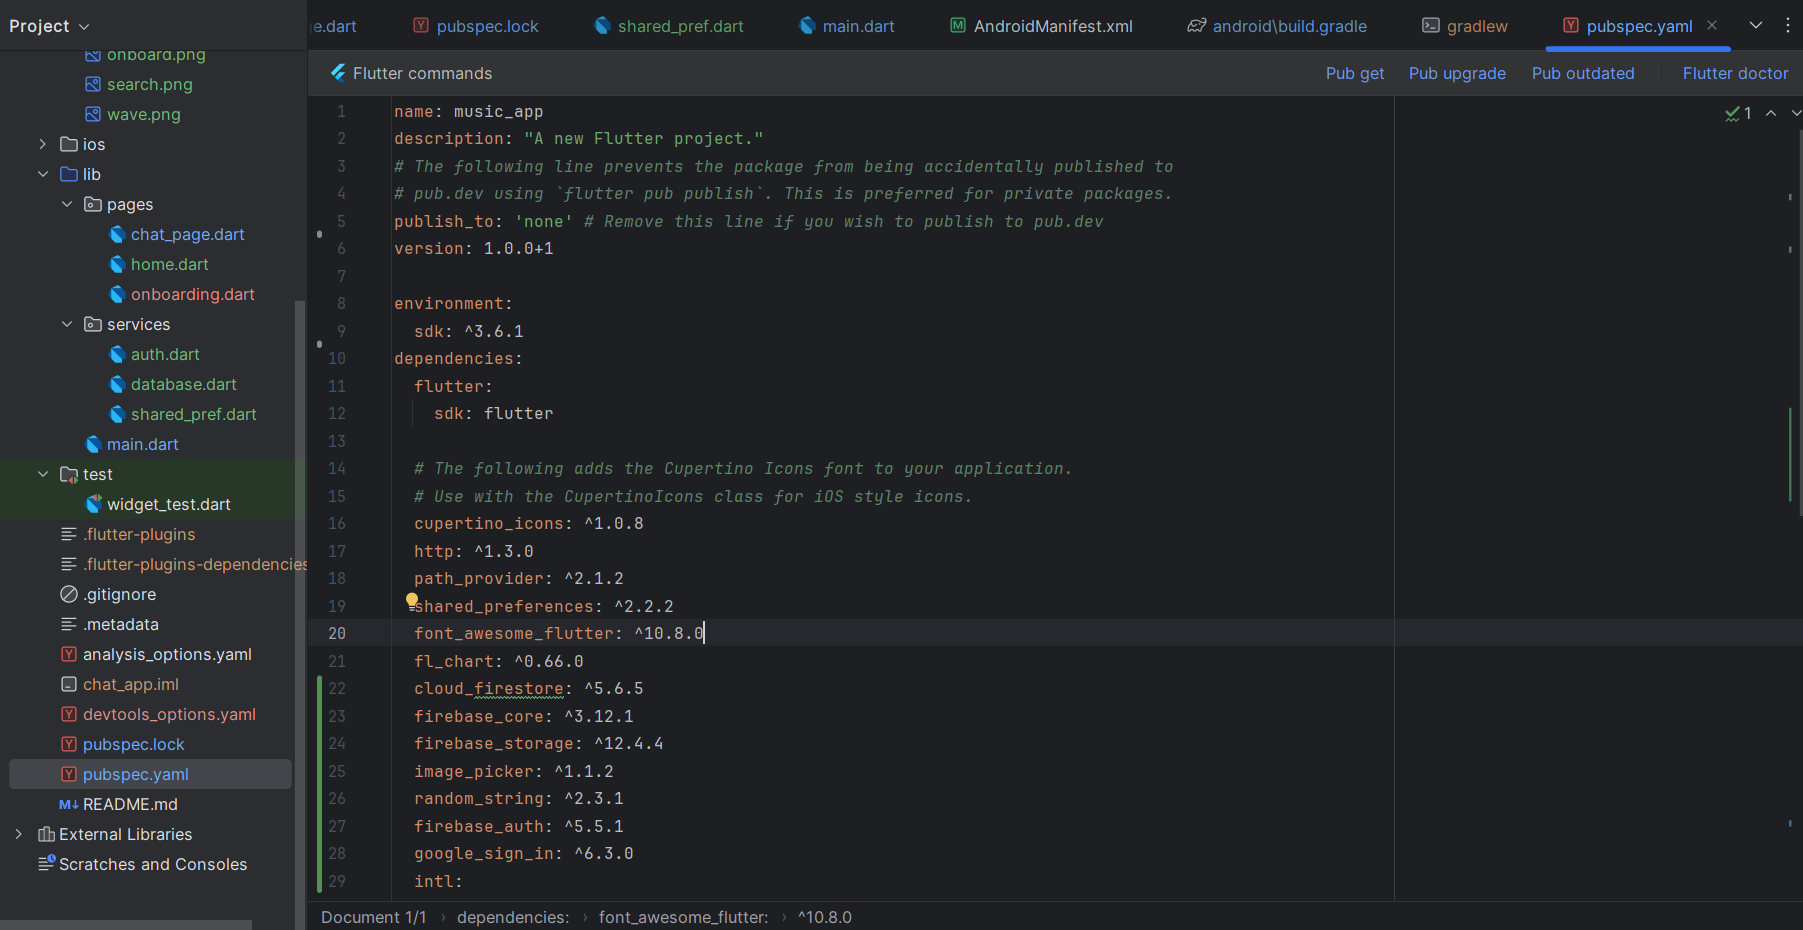
\includegraphics[width=1\textwidth]{Hinhve/pubspec.png}
    \caption{Hình ảnh nội dung file pubspec.yaml trong project thực tế}
    \label{fig:pubspec.png}
\end{figure}

Trong \textbf{pubspec.yaml}, các trường \texttt{metadata} chính thường gặp bao gồm:
\begin{itemize}
    \item \texttt{name}: Tên của package (bắt buộc phải có cho mọi gói Dart). \\
    Ví dụ: \texttt{name: music\_app}
    \item \texttt{version}: Phiên bản của gói \\
    Ví dụ: \texttt{version: 1.0.0+1}
    \item \texttt{description}: Mô tả ngắn gọn về gói hoặc dự án \\
    Ví dụ: \texttt{description: "A new flutter project"} 
    \item \texttt{dependencies}: Danh sách các gói khác mà gói này phụ thuộc. Nếu dự án không dùng gói ngoài nào thì phần này có thể để trống hoặc không khai báo. Trong dependencies, mỗi mục là tên gói và phiên bản tương thích. \\
    Ví dụ: \\
    \texttt{dependencies:} \\
        \texttt{cupertino\_icons: \^{}1.0.8} \\
        \texttt{http: \^{}1.3.0}
\end{itemize} 

Ngoài ra, còn có các trường thông tin khác như \texttt{homepage, repository, environment,...} tùy nhu cầu dự án. 

\textbf{Cách sử dụng các lệnh import trong Dart:} 

Để sử dụng các thư viện trong mã Dart, cú pháp chung là \texttt{import 'uri'}. Có 3 dạng \texttt{uri} chính:
\begin{itemize}
\item \textbf{Thư viện chuẩn của Dart: } Ví dụ \texttt{dart:core, dart:math, dart:convert, dart:io,...}. Những thư viện này cung cấp các chức năng cơ bản và thường được nhập tự động. 
Ví dụ, thư viện toán học được import bằng \texttt{import 'dart:math';} để sử dụng các hàm như $sqrt$ hoặc hằng số $\pi$.
\begin{lstlisting}
import 'dart:math';
    void main() {
    int a = 4;
    double b = 2.0;
    print('${sqrt(a)}'); 
    print('${max(a, b)}');
}
/*
2
4
*/
\end{lstlisting}
    \item \textbf{Tệp nguồn nội bộ (file dự án):} Sử dụng đường dẫn tương đối hoặc tuyệt đối đến file Dart trong dự án. \\
    Ví dụ, \texttt{import 'lib/myfile.dart'} sẽ nạp file \texttt{myfile.dart} nằm trong thư mục \texttt{lib/}
    \item \textbf{Thư viện từ gói tải về (packages):} Dùng định danh theo dạng package: \texttt{package:<ten\_goi>/<thu\_vien\_goi>} \\
    Ví dụ, gói \texttt{googleapis\_auth} có thành phần \texttt{auth\_browser} cung cấp chức năng xác thực Auth với tài khoản Google thì nạp thư viện đó vào bằng: \\
    \texttt{import "package:googleapis\_auth/auth\_browser.dart"}
\end{itemize}

\textbf{Một số thư viện chuẩn phổ biến trong Dart:} 

Dart cung cấp một loạt thư viện mặc định (bắt đầu bằng \texttt{dart:}) để xử lý nhiều tác vụ thông thường. Các thư viện quan trọng bao gồm:
\begin{itemize}
\item \texttt{dart:core}:  Thư viện lõi cung cấp các kiểu dữ liệu cơ bản và hàm tiện ích.

\textit{Ví dụ:}
\begin{lstlisting}
void main() {
  String name = 'Khanh';
  int age = 20;
  print('Name: $name, Age: $age');

  var now = DateTime.now();
  var later = now.add(Duration(days: 2));
  print('Two days later is: $later');
}
/*
Name: Khanh, Age: 20
Two days later is: 2025-05-02 07:34:20.215
*/
\end{lstlisting}

\item \texttt{dart:collection}: Cung cấp các cấu trúc dữ liệu nâng cao như \textbf{HashSet, HashMap, Queue…} phục vụ lưu trữ và truy vấn dữ liệu động.

\textit{Ví dụ về \textbf{Queue}:}

\begin{lstlisting}
import 'dart:collection';
void main() {
  Queue<String> queue = Queue();
  queue.addAll(['one', 'two', 'three']);
  print(queue.removeFirst()); // one
  print(queue);               // (two, three)
}
\end{lstlisting}

Ví dụ về \textbf{SplayTreeSet}:
\begin{lstlisting}[language=Dart]
// Import the collection library for SplayTreeSet
import 'dart:collection';

void main() {
  // Create a SplayTreeSet of integers
  var evenNumbers = SplayTreeSet<int>();
  evenNumbers.addAll([10, 2, 6, 4, 8]);

  print('Set after adding elements:');
  for (var x in evenNumbers) {
    print(x); 
  }

  // Remove the value 6
  evenNumbers.remove(6);
  print('\nAfter removing number 6:');
  print(evenNumbers);

  // Display the smallest and largest values
  print('\nSmallest number: ${evenNumbers.first}');
  print('Largest number: ${evenNumbers.last}');
}
\end{lstlisting}

Kết quả của chương trình trên in ra là:
\begin{myverbatim}
Set after adding elements:
2
4
6
8
10

After removing number 6:
{2, 4, 8, 10}

Smallest number: 2
Largest number: 10
\end{myverbatim}
\item \texttt{dart:math}: Thư viện toán học chứa các hàm và các hằng số cơ bản.

\textit{Ví dụ:}

\begin{lstlisting}
import 'dart:math';

void main() {
  print(pi);             // 3.141592...
  print(sqrt(49));       // 7.0
  print(pow(3, 3));      // 27

  // Print a random integer from 0 to 9
  print(Random().nextInt(10)); 
}
\end{lstlisting}

\item \texttt{dart:convert}: Cung cấp bộ mã hóa và giải mã dữ liệu, hỗ trợ JSON, UTF-8, và các định dạng dữ liệu khác.

\textit{Ví dụ về chuyển đổi từ \textbf{Map} thành \textbf{JSON}:}
\begin{lstlisting}
import 'dart:convert';
void main() {
  var user = {'name': 'Hai', 'age': 22};
  var jsonStr = jsonEncode(user);
  print(jsonStr); // {"name":"Hai","age":22}
}
\end{lstlisting}

\textit{Ví dụ giải mã từ \textbf{JSON}:}

\begin{lstlisting}[language=Dart]
import 'dart:convert';
void main() {
  var jsonStr = '{"name" : "Hai","age" : 22}';
  var user = jsonDecode(jsonStr);
  print(user['name']); // Hai
}
\end{lstlisting}

\textit{Ví dụ về mã hóa và giải mã \textbf{Base64}:}
\begin{lstlisting}
import 'dart:convert';
void main() {
  var message = 'Dart';
  var bytes = utf8.encode(message);
  var base64Str = base64Encode(bytes);
  print(base64Str); // RGFydA==

  var x = utf8.decode(base64Decode(base64Str));
  print(x); // Dart
}
\end{lstlisting}

\item \texttt{dart:io}: Thư viện nhập xuất cho chương trình chạy trên máy (VM), hỗ trợ thao tác file, socket, HTTP,...

\item \texttt{dart:js, dart:html}: Các thư viện phục vụ lập trình Web. Trong đó \texttt{dart:html} cho phép thao tác DOM và API HTML5 trên trình duyệt, còn \texttt{dart:js} hỗ trợ tương tác với mã JavaScript.
\end{itemize}
\end{document}